\label{ch:AnalysingGraphs}

\begin{jointwork}
	In this chapter, we will put the tools and workflows described in the previous sections to the use. We will train an RL agent, and then monitor it using all the tools at our disposal, highlighting where each tool is most useful, and what could be improved.
\end{jointwork}

\section{Setting up the experiment}

% Before starting our monitoring, we will be conducting two different experiments, each with a different RL algorithm and a different market environment. Both experiments will however be conducted on the same marketplace type, a Circular Economy model with rebuy prices. To ensure that we are evaluating an agent with a performance that is to be expected with the provided parameters after the experiments have finished, we will run both the experiments multiple times to be able to identify outliers in the data. Diagrams of different versions of an experiment will be denoted using an underscore for differentiation.

% \subsection*{SAC-Duopoly}

% For the first experiment, we will train an RL agent using the SAC-algorithm~\cite{StableBaselines3SAC} on a Duopoly marketplace with rebuy prices. The agent will be trained against a rule-based agent, more specifically the \emph{RuleBasedCERebuyAgentCompetitive}, as presented in \bfref{subsec:DataDrivenModels}. The configuration files for this experiment can be found in \Cref{fig:SACDuopolyConfigEnvironment}, \Cref{fig:SACDuopolyConfigMarket} and \Cref{fig:SACDuopolyConfigAgent}. We will refer to this experiment as the \emph{SAC-Duopoly}.

%% Text for only one experiment
Before starting our monitoring, we will need to conduct an experiment, where an RL algorithm is being trained on a market environment. For our experiment, we will train an RL agent using the SAC-algorithm~\cite{StableBaselines3SAC} on a Duopoly marketplace with rebuy prices. The agent will be trained playing against a rule-based agent, more specifically the \emph{RuleBasedCERebuyAgentCompetitive}, as presented in \bfref{subsec:DataDrivenModels}. The configuration files for this experiment can be found in \Cref{fig:SACDuopolyConfigEnvironment}, \Cref{fig:SACDuopolyConfigMarket} and \Cref{fig:SACDuopolyConfigAgent}. We will refer to this experiment as the \emph{SAC-Duopoly} experiment. To ensure that we are evaluating an agent with a performance that is to be expected with the provided parameters, we will conduct the experiment multiple times to be able to identify outliers in the data. All diagrams except those shown in \Cref{fig:SACDuopolyProfitsMean} (which contains diagrams from each of the four experiment runs) have been taken from the same experiment run, denoted as \emph{SAC-Duopoly\_1} in \Cref{fig:SACDuopolyProfitsMean1}.

For the interested reader, a number of diagrams created through a second experiment are available in the Appendix under \bfref{sec:AppendixOligopolyDiagrams}. In this second experiment, a PPO-Agent (see \bfref{item:StableBaselines}) was trained against four rule-based competitors on a Circular Economy market with rebuy prices. The configuration files for this experiment can be found in \bfref{sec:AppendixOligopolyConfig}.

% \subsection*{PPO-Oligopoly}

% For the second experiment, we will be training a different RL agent on a more complex market with more participants: A PPO-agent~\cite{StableBaselines3PPO} will be trained on an Oligopoly-Scenario, again with rebuy prices enabled. Three different rule-based agents will compete against the PPO-Agent on the same market:

% \begin{enumerate}
% 	\item A \emph{FixedPriceAgent}, which will always set the following three prices:
% 	      \begin{itemize}
% 		      \item New price: 7
% 		      \item Refurbished price: 4
% 		      \item Rebuy price: 2
% 	      \end{itemize}
% 	      It should be noted that the configured maximum possible price is 10, which can also be configured using the configuration files. Depending on this maximum price, the prices set by \emph{FixedPriceAgents} must be adjusted to allow them to realistically compete in the market.
% 	\item The second agent is a \emph{RuleBasedCERebuyAgentCompetitive}, a more complicated and sophisticated version of the simple \emph{RuleBasedCERebuyAgent}, which was introduced in \bfref{subsec:InventoryBasedModels}. The competitive version used for this experiment combines features of both the basic \emph{RuleBasedCERebuyAgent} and the \emph{RuleBasedCERebuyAgentStorageMinimizer}. It's policy implementation can be found in \todo{Insert code snippet in Appendix}xyz.\todo{Check if the agents are correct/order is correct}
% 	\item For the third competitor, we will again be using the \emph{RuleBasedCERebuyAgentStorageMinimizer}.
% \end{enumerate}
% This experiment will be referred to as the \emph{PPO-Oligopoly}.\todo{Config files for experiment, reuse same market config figure.}

\section{Experiment results}

In the following sections we will use our different monitoring tools on the results of the SAC-Duopoly experiment. We will start with the Live-monitoring tool, which runs automatically after the training run has completed and creates over 90 graphs and diagrams already. Due to this high number of available diagrams, we will always only look at a curated selection, highlighting those which give the best insights into the trained agent.

\subsection{Live- and Agent-monitoring}\label{subsec:LiveMonitoringResults}

\begin{figure}[t]
	\centering
	\begin{subfigure}{0.49\textwidth}
		\centering
		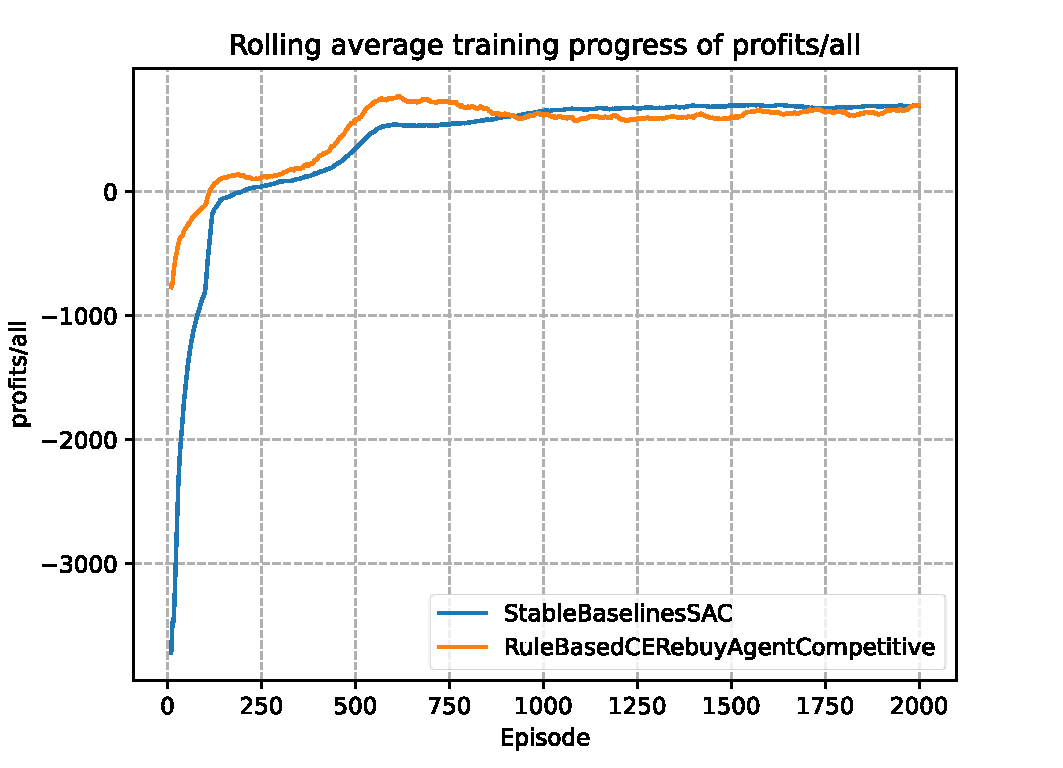
\includegraphics[width = \textwidth]{images/experiments/SACDuopoly/SACDuopolyProfitsMean1.pdf}\\
		\subcaption{SAC-Duopoly\_1, 2,000 training episodes}\label{fig:SACDuopolyProfitsMean1}
	\end{subfigure}
	\begin{subfigure}{0.49\textwidth}
		\centering
		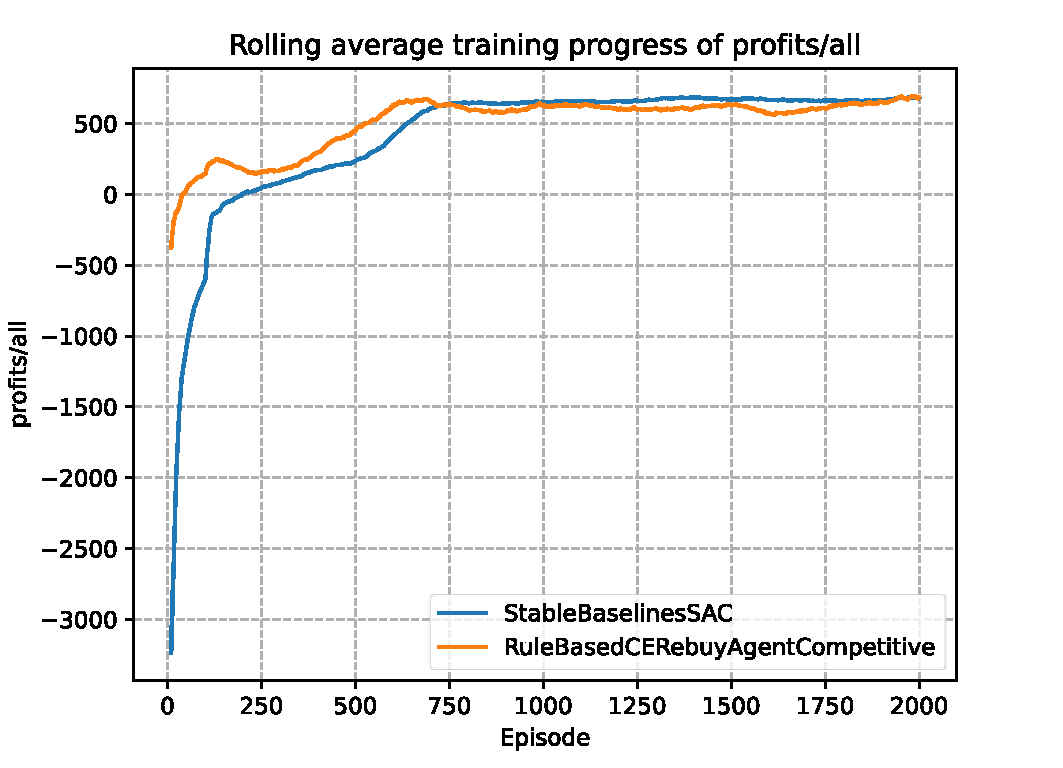
\includegraphics[width = \textwidth]{images/experiments/SACDuopoly/SACDuopolyProfitsMean2.pdf}\\
		\subcaption{SAC-Duopoly\_2, 2,000 training episodes}\label{fig:SACDuopolyProfitsMean2}
	\end{subfigure}
	\begin{subfigure}{0.49\textwidth}
		\centering
		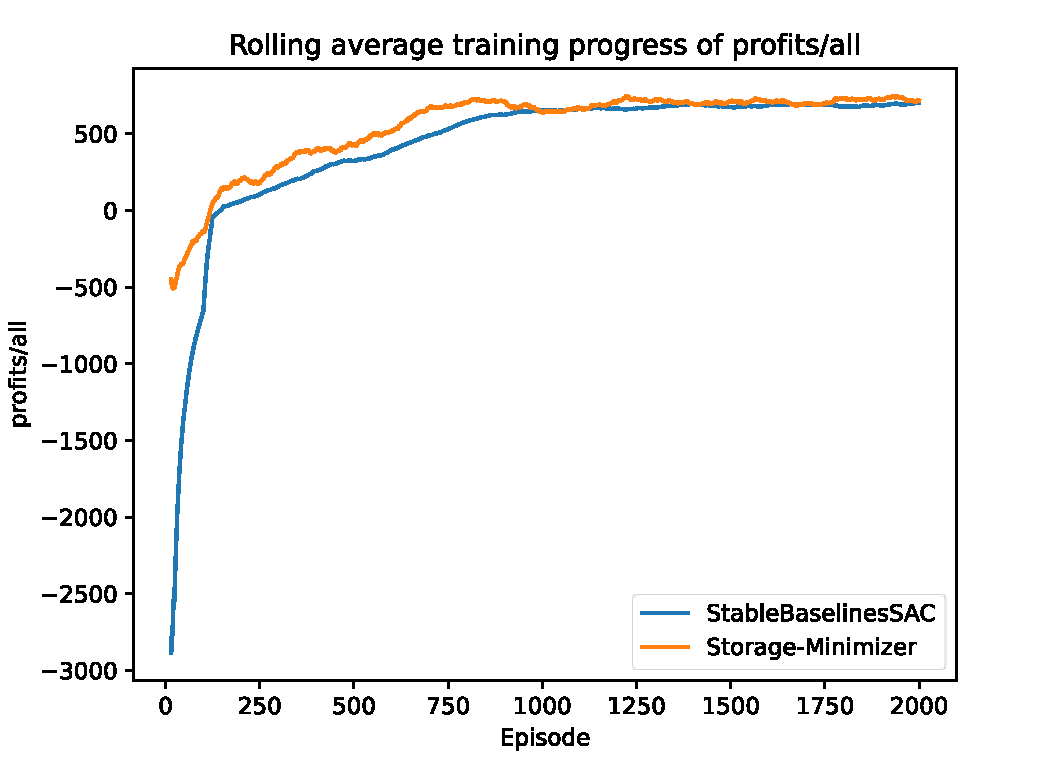
\includegraphics[width = \textwidth]{images/experiments/SACDuopoly/SACDuopolyProfitsMean3.pdf}\\
		\subcaption{SAC-Duopoly\_3, 2,000 training episodes}\label{fig:SACDuopolyProfitsMean3}
	\end{subfigure}
	\begin{subfigure}{0.49\textwidth}
		\centering
		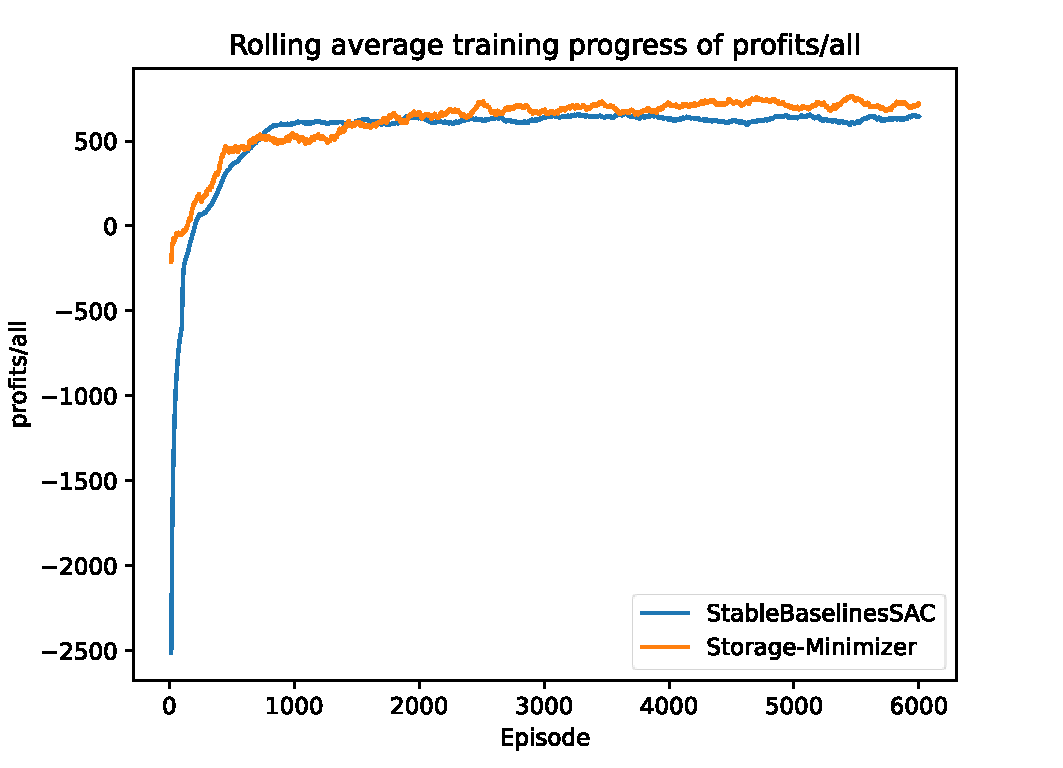
\includegraphics[width = \textwidth]{images/experiments/SACDuopoly/SACDuopolyProfitsMean4.pdf}\\
		\subcaption{SAC-Duopoly\_4, 6,000 training episodes}\label{fig:SACDuopolyProfitsMean4}
	\end{subfigure}
	\caption{Profit per episode of four different training runs of an SAC-Agent on a Duopoly market.}\label{fig:SACDuopolyProfitsMean}
\end{figure}

This section will focus on the diagrams created by the Live-monitoring tool after training, which always runs an Agent-monitoring session as well, to immediately provide the user with many additional useful diagrams without the need to run the tool manually.

A commonly asked question when deciding on the quality of an RL agent is their \emph{stability}. If an algorithm is stable, the trained agent will produce similar results over multiple training sessions, on the condition that the parameters do not differ. Not only the rewards achieved at the end of the training will be very similar, but also the amount of episodes needed to reach certain thresholds. In the case of the SAC-Duopoly experiment, we ran the same configuration four times: The first three experiments were run using the exact same parameters, for the fourth experiment the amount of training episodes were tripled, meaning that the SAC-Agent had more time to alter its policy. \Cref{fig:SACDuopolyProfitsMean} shows the results of these four training sessions, created using the Live-monitoring tool and visualises the data collected during the training process. Although many other graphs are created (\Cref{tab:AllMetrics}), the visualisation of the total profit of the agent is the most convenient to use when evaluating an agent's performance, as the total profit is the parameter which the agent is trying to optimize.

\Cref{fig:SACDuopolyProfitsMean} shows the stability of the SAC-Agent very well. The agent not only reached the break-even threshold of a reward of 0 after around 150 episodes in each of the four training runs, but no matter the total length of training (see the model in \Cref{fig:SACDuopolyProfitsDensity4}, which was trained three times as long as the others), the profit would always stabilize and stay at around 670. Had the monitoring tools shown that the agent performs worse than expected in some of the experiments, we could conclude that this particular algorithm is not fit for the type of work required by our market simulation.

We can also observe that the profits of the SAC-Agent and the rule-based agent (in the case of this experiment, a \emph{RuleBasedCERebuyAgentStorageMinimizer}) seem to be closely linked to each other in this particular scenario. In the beginning of each experiment, when the RL agent still knows very little about the market and makes great losses, the rule-based agent also has a hard time to perform well. However, as soon as the SAC-Agent starts to perform better, the rule-based agent is also able to increase its mean profits at around the same rate as the SAC-Agent. Even more interestingly, the agents not only increase their profits at the same rate, but also very quickly arrive at a point where they earn the same mean amount as the other.

This might lead one to believe that the two competitors' policies align closely with each other. To validate this claim, another type of diagram created by the Live-monitoring tool can be used: The densityplots. These diagrams visualise probability densities for the various datasets recorded. While the diagrams shown in \Cref{fig:SACDuopolyProfitsMean} simply visualise data that was collected during the training run, densityplots are created by running the Agent-monitoring tool, where the marketplace is simulated an additional time. This allows us to use the `intermediate' models we saved during the training run (see \bfref{subsec:LiveMonitoring}) to compare the RL agent's policies at different points in time during the training.

\begin{figure}[t]
	\centering
	\begin{subfigure}{0.49\textwidth}
		\centering
		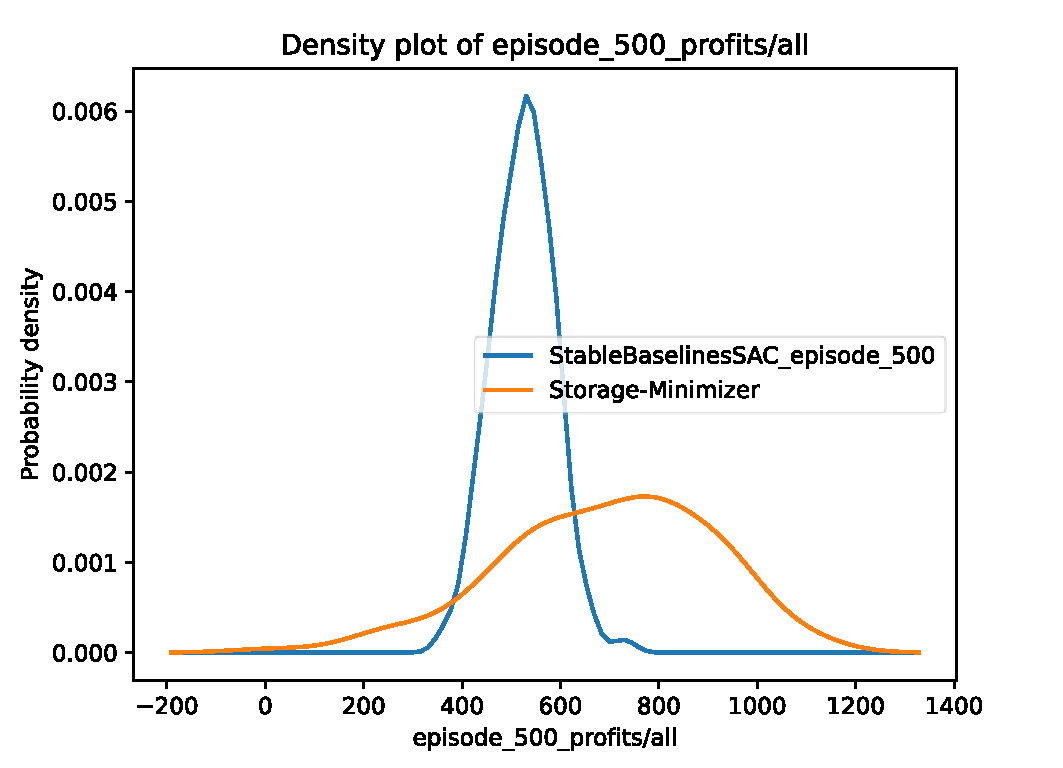
\includegraphics[width = \textwidth]{images/experiments/SACDuopoly/SACDuopolyProfitsDensity1.pdf}\\
		\subcaption{Model trained for 500 episodes}\label{fig:SACDuopolyProfitsDensity1}
	\end{subfigure}
	\begin{subfigure}{0.49\textwidth}
		\centering
		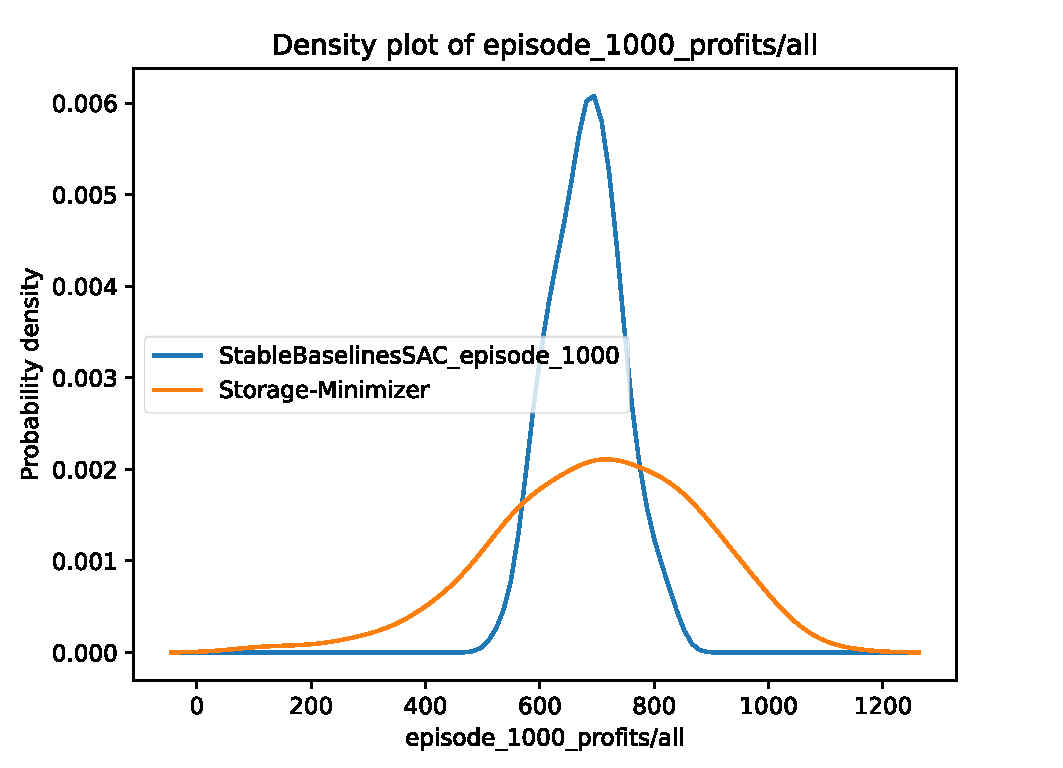
\includegraphics[width = \textwidth]{images/experiments/SACDuopoly/SACDuopolyProfitsDensity2.pdf}\\
		\subcaption{Model trained for 1,000 episodes}\label{fig:SACDuopolyProfitsDensity2}
	\end{subfigure}
	\begin{subfigure}{0.49\textwidth}
		\centering
		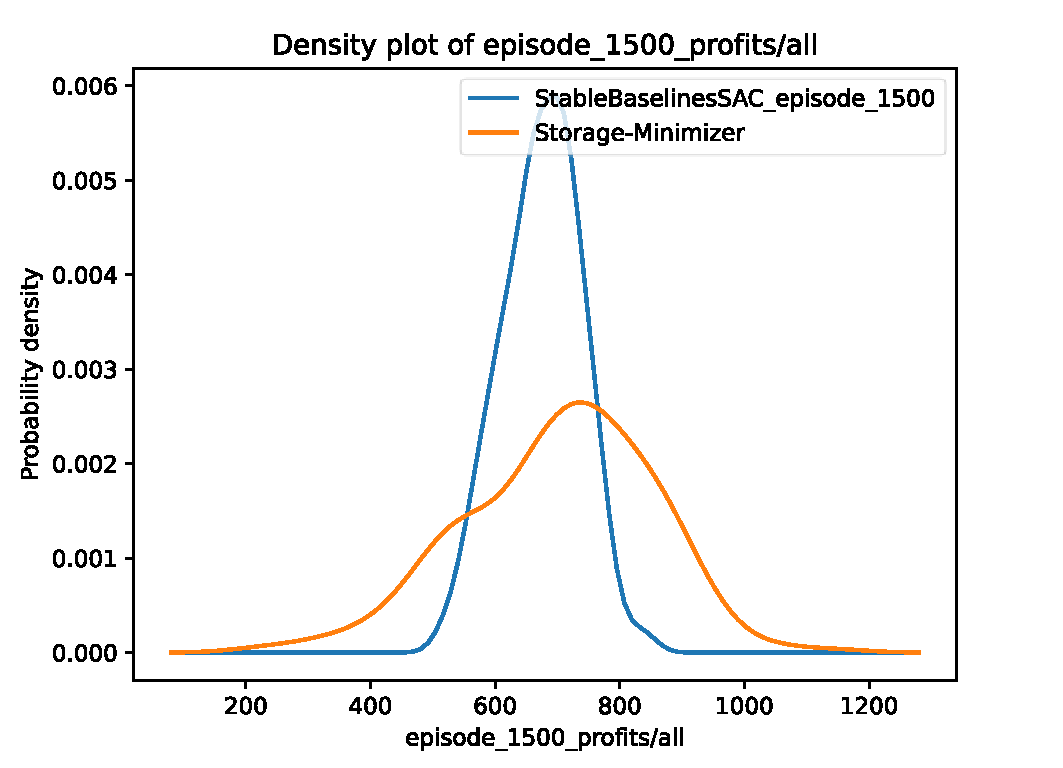
\includegraphics[width = \textwidth]{images/experiments/SACDuopoly/SACDuopolyProfitsDensity3.pdf}\\
		\subcaption{Model trained for 1,500 episodes}\label{fig:SACDuopolyProfitsDensity3}
	\end{subfigure}
	\begin{subfigure}{0.49\textwidth}
		\centering
		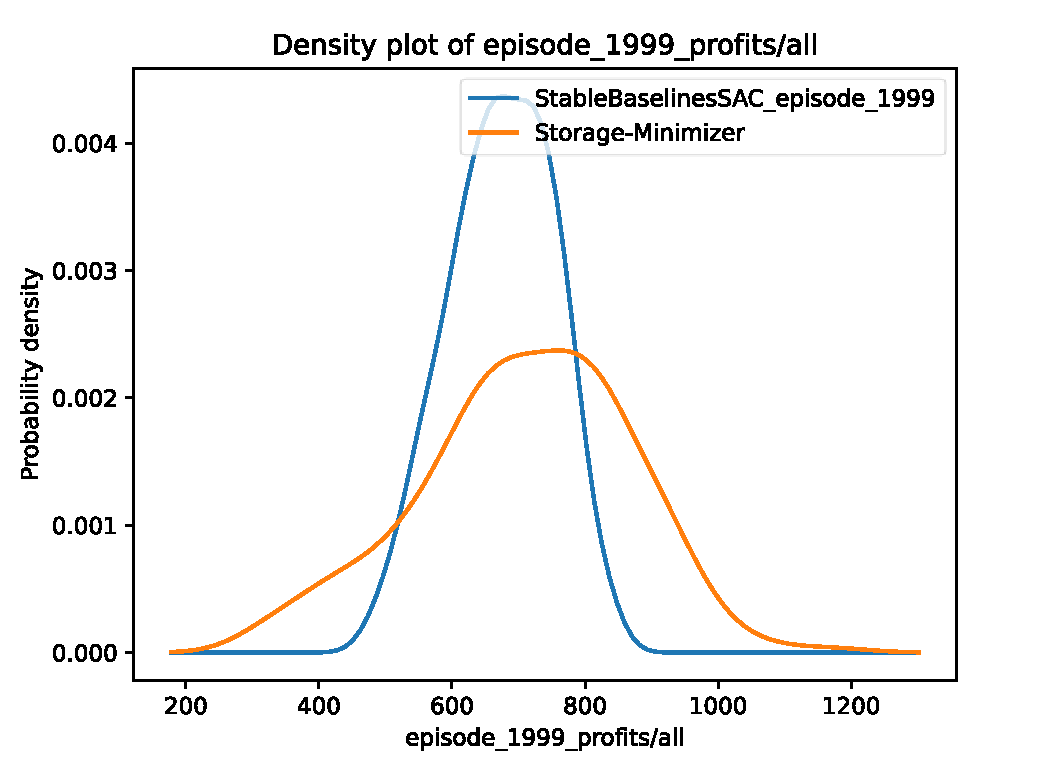
\includegraphics[width = \textwidth]{images/experiments/SACDuopoly/SACDuopolyProfitsDensity4.pdf}\\
		\subcaption{Model trained for 2,000 episodes}\label{fig:SACDuopolyProfitsDensity4}
	\end{subfigure}
	\caption{Probability densities for achieving a certain profit for four different training stages of the model trained during the \emph{SAC-Duopoly\_1} experiment.}\label{fig:SACDuopolyProfitsDensity}
\end{figure}

\Cref{fig:SACDuopolyProfitsDensity} shows the densityplots of profit-per-episode for four different training stages of the \emph{SAC-Duopoly\_1} experiment. From this it can be concluded that the claim that the two competitors' policies align closely is incorrect: even though the mean reward within an episode is always very similar (\Cref{fig:SACDuopolyProfitsMean1}), the SAC-Agent achieves rewards which lie closer together, while the rule-based agent's rewards have more of a spread.

We can also observe that the models which were trained for longer are not necessarily better or even the same quality of the models with less experience. There is a significant improvement going from the model shown in \Cref{fig:SACDuopolyProfitsDensity1} to the one in \Cref{fig:SACDuopolyProfitsDensity2}, this shift in the probability density curve can be correlated with the maximum mean rewards the two models could achieve during the training: For the model trained for 500 episodes, this was around 450, for the other it was about 660 (\Cref{fig:SACDuopolyProfitsMean1}). Both of these values have respectively high probabilities of being reached during the second simulation after the training has concluded, i case of the model trained for 1,000 episodes, this even coincides with the maximum in the density plot (\Cref{fig:SACDuopolyProfitsDensity2}). Going from the model trained for 1,000 episodes to the next one, which was trained for 1,500 episodes (\Cref{fig:SACDuopolyProfitsDensity3}), both the probability densities and the mean rewards stay very close to each other. From this we can conclude that training the SAC-Agent for more than 1,000 episodes is very likely to not have a great effect on the maximum reward achievable by the algorithm. Going from the model trained for 1,500 episodes to the last one, saved at the end of the training (\Cref{fig:SACDuopolyProfitsDensity4}), we can however see a deterioration in performance: While the mean rewards hardly changed (see \Cref{fig:SACDuopolyProfitsMean1}), the probability density curve got wider at its base, extending out further towards a reward of 400, and lowering the probability of achieving a reward of 700 from previously above 0.5\% to under 0.4\%. This means that the model which was trained for the longest time produces less predictable results than those trained less, which is a tame version of so-called \emph{Catastrophic Forgetting}, which will be explained further in \bfref{subsec:FutureLiveMonitoring}. The insights gained by our monitoring tools combined with the fact that we save `intermediate' models of the RL agent during training allows us to find the optimal trained model to use for further investigation and eventual deployment in the real market. In the case of the \emph{SAC-Duopoly\_1} experiment, the optimal model would be the one trained for 1,000 episodes.

\subsection{Further investigation}

Besides the mean profits achieved during training, our Live-monitoring tool offers many other useful diagrams as well, a selection of which will be shown in this section. The graphs used will be from the \emph{SAC-Duopoly\_1} experiment.

Users may ask themselves how the profits achieved by the different vendors are split between the two available retail channels of new and refurbished products, how many products were bought back from customers or how much the vendors had to pay for storage of these used products. For all of these questions, the Live-monitoring (together with the Agent-monitoring) tool offers two types of diagrams: First, simple lineplots as shown in \Cref{fig:SACDuopolyProfitsMean} can be used, as well as scatterplots which visualise the exact data recorded during the episode, instead of the trends shown by the lineplots. \Cref{fig:SACDuopolyMixedGraphs} shows a number of different metrics, all of which are available as both linepots and scatterplots (see \Cref{tab:AllMetrics} for a list of all metrics and visualisations).

\begin{figure}[t]
	\centering
	\begin{subfigure}{0.49\textwidth}
		\centering
		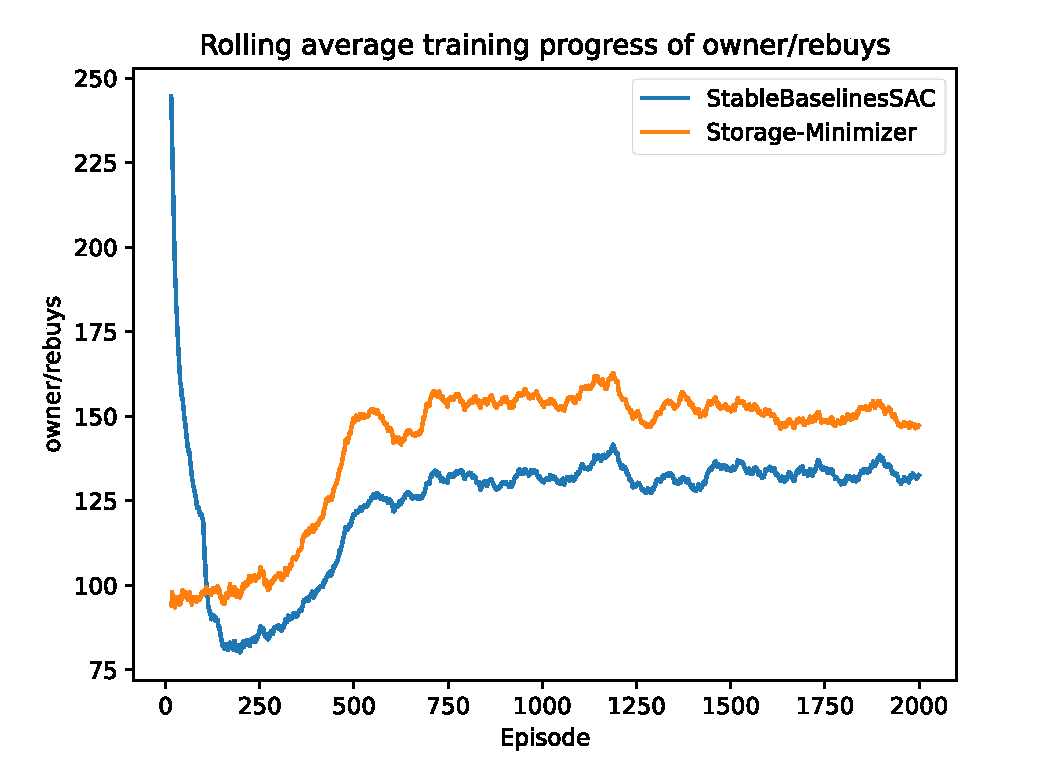
\includegraphics[width = \textwidth]{images/experiments/SACDuopoly/SACDuopolyMixedGraphs1.pdf}\\
		\subcaption{Storage costs for bought back products}\label{fig:SACDuopolyMixedGraphs1}
	\end{subfigure}
	\begin{subfigure}{0.49\textwidth}
		\centering
		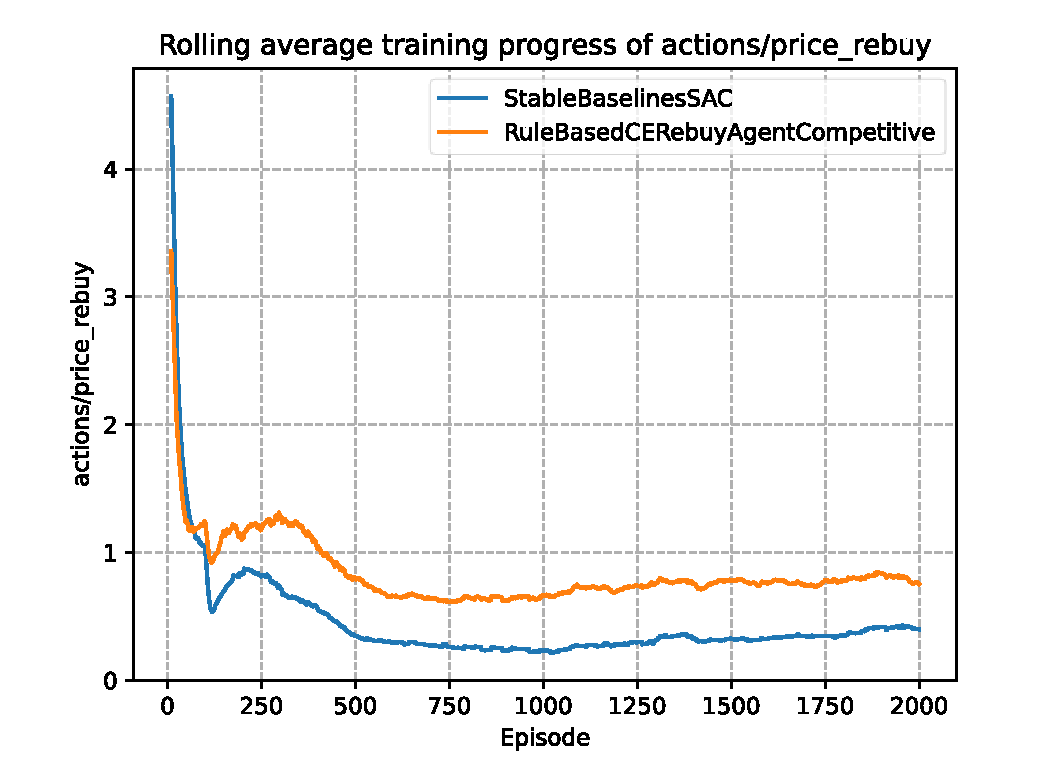
\includegraphics[width = \textwidth]{images/experiments/SACDuopoly/SACDuopolyMixedGraphs2.pdf}\\
		\subcaption{Rebuy prices set by the vendors}\label{fig:SACDuopolyMixedGraphs2}
	\end{subfigure}
	\begin{subfigure}{0.49\textwidth}
		\centering
		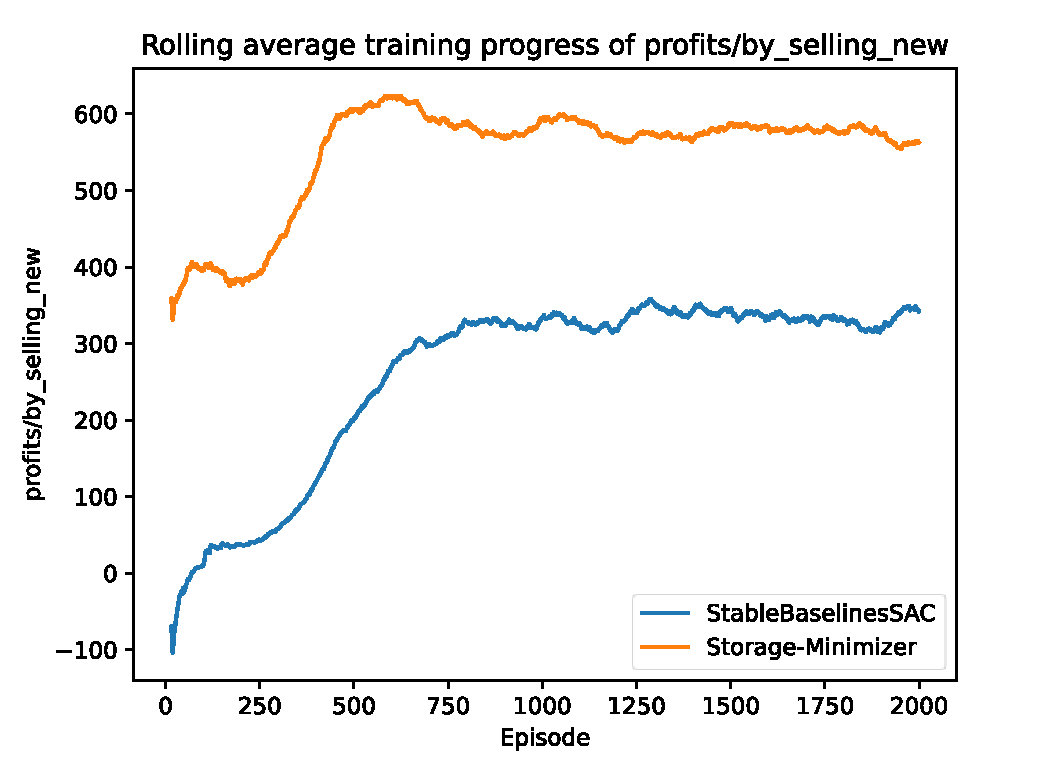
\includegraphics[width = \textwidth]{images/experiments/SACDuopoly/SACDuopolyMixedGraphs3.pdf}\\
		\subcaption{Customers that bought nothing}\label{fig:SACDuopolyMixedGraphs3}
	\end{subfigure}
	\begin{subfigure}{0.49\textwidth}
		\centering
		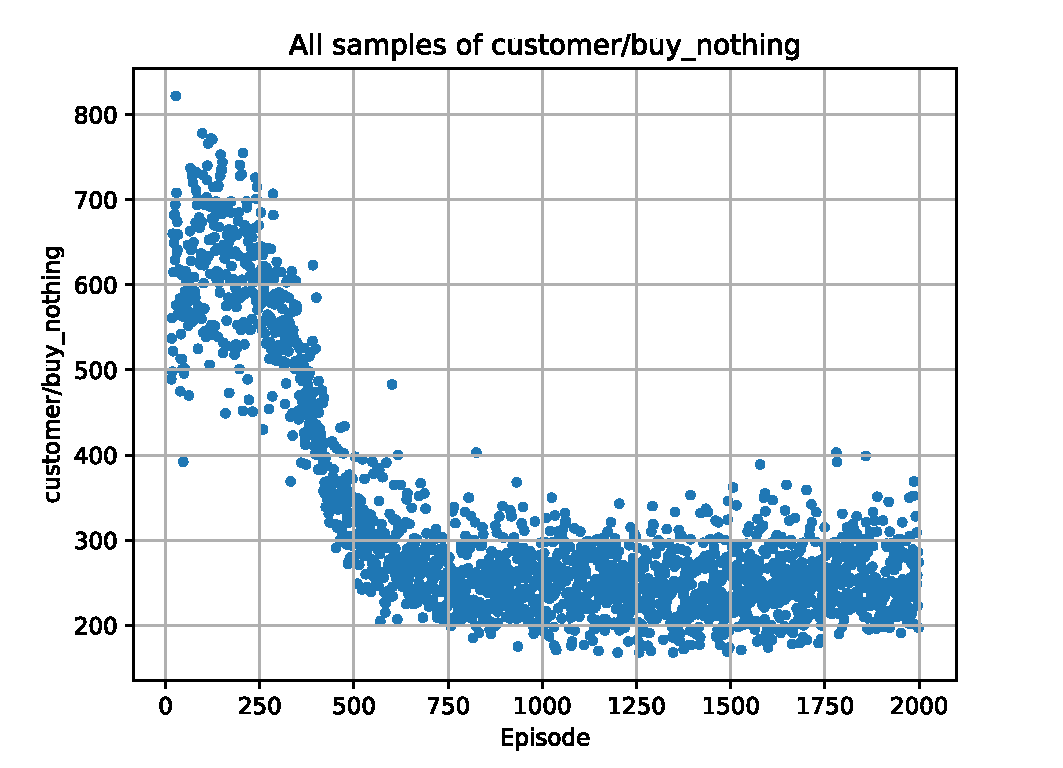
\includegraphics[width = \textwidth]{images/experiments/SACDuopoly/SACDuopolyMixedGraphs4.pdf}\\
		\subcaption{New prices set by the vendors}\label{fig:SACDuopolyMixedGraphs4}
	\end{subfigure}
	\caption{Diagrams visualising various data points collected during training of the \emph{SAC-Duopoly\_1} experiment.}\label{fig:SACDuopolyMixedGraphs}
\end{figure}

Many connections can be made when evaluating different diagrams side-by-side, such as the observation of the initially high storage costs of both vendors in \Cref{fig:SACDuopolyMixedGraphs1} being caused by high rebuy prices set by the agents (\Cref{fig:SACDuopolyMixedGraphs2}). High rebuy prices make it likely that customers are willing to sell back their products, which leads to (over)full inventories and high storage costs. High storage and rebuy costs will have then caused a policy change to set lower rebuy prices, thereby de-incentivizing customers to sell back as many products as they used to and lowering the agent's storage costs, increasing the profit margin.

The next pair of diagrams shows the connection between a high number of customer that buy nothing, as visualised in \Cref{fig:SACDuopolyMixedGraphs3} correlating to high prices for new products, shown in \Cref{fig:SACDuopolyMixedGraphs4}. As mentioned in \bfref{sec:Customers}, the customers implemented in our framework make their purchase decisions based on the prices they are presented with, which leads to many customers choosing to buy nothing before paying prices as high as set by the vendors.
% The next pair of diagrams tells us two things: First, the vendors' initially low profits from selling new products as shown in \Cref{fig:SACDuopolyMixedGraphs3}, or in the bigger picture, low profits overall (\Cref{fig:SACDuopolyProfitsMean1}) were not caused by the vendors setting prices that are too low, but rather too high. This is confirmed by an initially very high number of customers which chose to not buy any of the products offered by the vendors (\Cref{fig:SACDuopolyMixedGraphs4}). Additionally, when comparing the total profits of the two vendors with the profits gained from selling only new products (\Cref{fig:SACDuopolyProfitsMean1} and \Cref{fig:SACDuopolyMixedGraphs3}), we can come to the conclusion that the SAC-Agent must have learned to prioritize selling refurbished products over new ones and keeping storage costs low, since we know that overall profits for the two vendors are about the same in the later parts of the training, but the SAC-Agent sells a lot less new products than its rule-based counterpart.

If the Agent-monitoring is run after a training session (with a number of intermediate models), it also creates violinplots for all of the collected metrics (\Cref{tab:AllMetrics}). A selection of such diagrams can be found in \Cref{fig:SACDuopolyViolinPlots}, showing the respective total profits (\Cref{fig:SACDuopolyViolinPlots1}) and storage costs (\Cref{fig:SACDuopolyViolinPlots2}) for each intermediate model of the trained SAC-Agent. As explained in \bfref{subsec:AgentMonitoring}, these plots visualise the probability distributions as shown in \Cref{fig:SACDuopolyProfitsDensity} in a more condensed way, providing additional data such as actual maximum, minimum and median values as well. The biggest upside of the Violinplots is however that they are able to show the distributions for all intermediate models in one diagram, which allows for even better comparisons. Looking at \Cref{fig:SACDuopolyViolinPlots1} we can immediately see the difference in the spread of total profits achieved between the models trained for 1,500 and 2,000 episodes respectively, for which we previously needed to consult and compare two different diagrams (\Cref{fig:SACDuopolyProfitsDensity3} and \Cref{fig:SACDuopolyProfitsDensity4}). Similarly, \Cref{fig:SACDuopolyViolinPlots2} is able to tell us something else we did not know before: the longer a model was trained for, the more likely it is that it will induce high storage costs, a trend which was not necessarily visible in \Cref{fig:SACDuopolyMixedGraphs1}.

Violinplots do however not replace the need for densityplots, as both have an equally useful way of displaying data. While the violinplots show rough distributions plotting against the real numbers on the y-axis, the densityplots show the concrete probability values for each possible data point.

\begin{figure}[t]
	\centering
	\begin{subfigure}{0.49\textwidth}
		\centering
		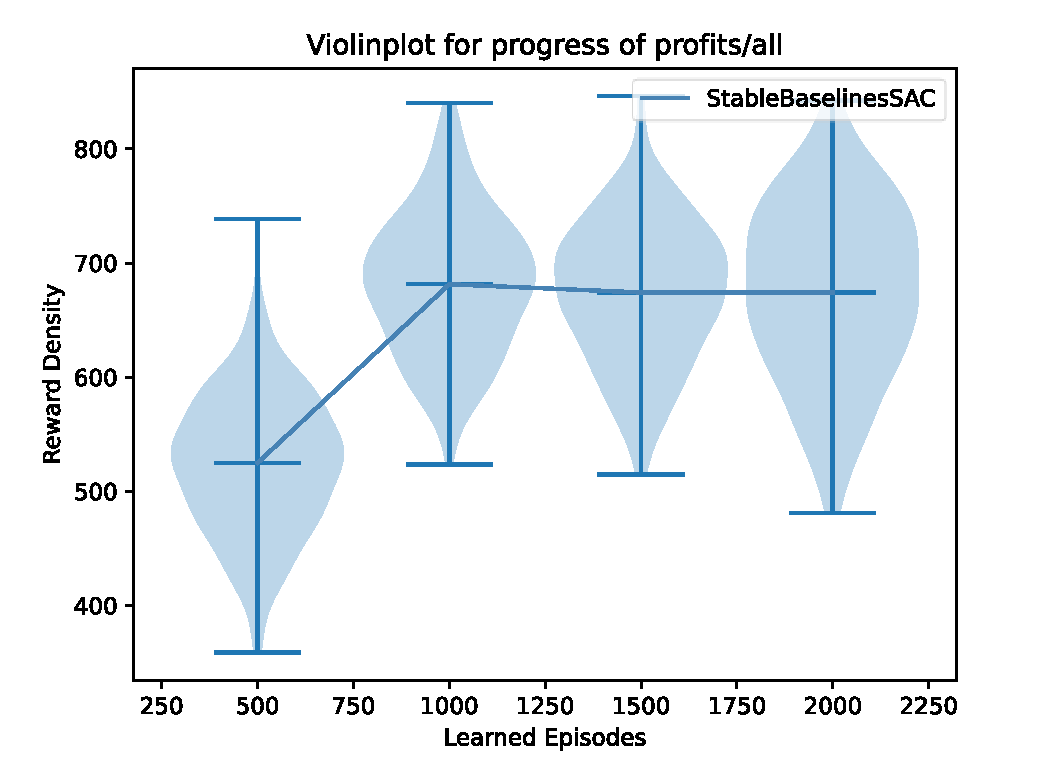
\includegraphics[width = \textwidth]{images/experiments/SACDuopoly/SACDuopolyProfitsAllViolin.pdf}\\
		\subcaption{Total profits for all intermediate models}\label{fig:SACDuopolyViolinPlots1}
	\end{subfigure}
	\begin{subfigure}{0.49\textwidth}
		\centering
		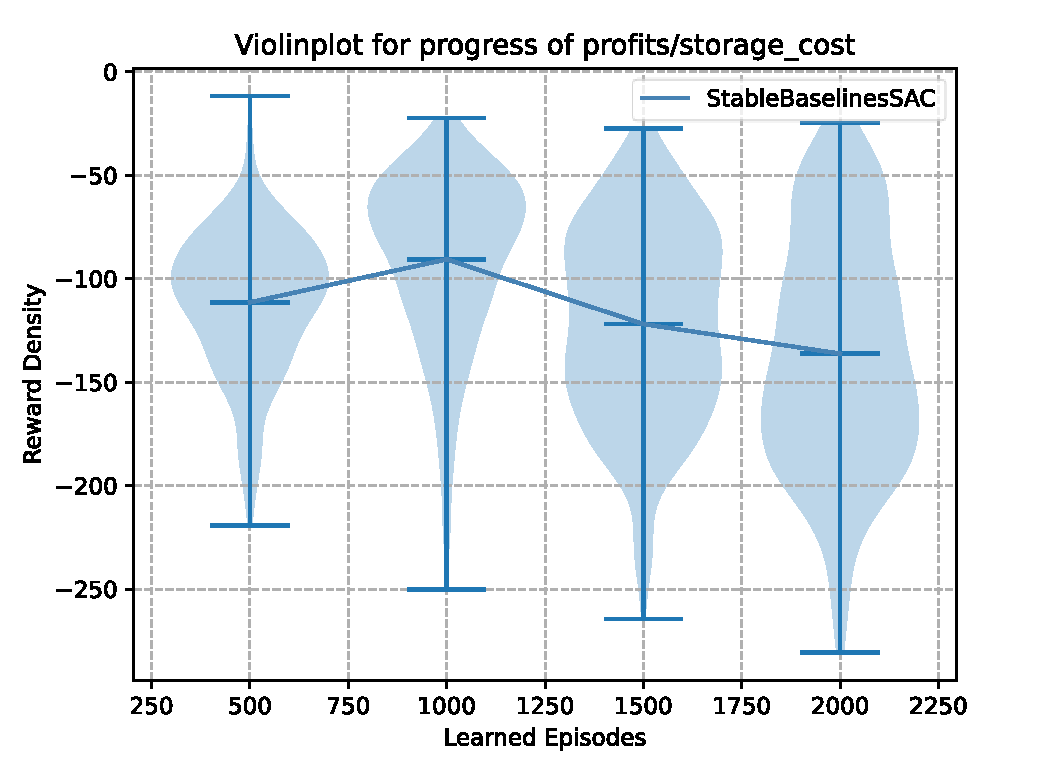
\includegraphics[width = \textwidth]{images/experiments/SACDuopoly/SACDuopolyStorageCostsViolin.pdf}\\
		\subcaption{Storage costs for all intermediate models}\label{fig:SACDuopolyViolinPlots2}
	\end{subfigure}
	\caption{Violinplots showing a selection of collected data when running Agent-monitoring after training.}\label{fig:SACDuopolyViolinPlots}
\end{figure}

\subsection{Exampleprinter}

All of the diagrams shown in the previous section were created as part of the automatic monitoring done after a training session has concluded. There are however two other tools at our disposal to monitor the trained RL agent after they have been trained. For this, we only need the intermediate models saved during and at the end of training. In the case of the \emph{SAC-Duopoly\_1} experiment, we will be using the model saved after 1,000 episodes, as we discovered it had the best performance, see \bfref{subsec:LiveMonitoringResults}. The first tool we will now utilize is the Exampleprinter, as introduced in \bfref{subsec:Exampleprinter}.

To configure this monitoring run, we will again need three configuration files: one defining the task to be done (for which we will re-use the one shown in \Cref{fig:SACDuopolyConfigEnvironment}, only exchanging the `task' keyword), and one for both the hyperparameter-configuration of the market and the SAC-Agent, for which we will also re-use the configuration files used for training (\Cref{fig:SACDuopolyConfigMarket} and \Cref{fig:SACDuopolyConfigAgent}). By using the same configuration files again, we can emulate the market the agent was initially trained on as closely as possible.

At the end of the monitoring session, we receive an animated overview diagram that cycles through all time steps, allowing us to identify and examine potentially interesting time steps in the simulation. Due to the nature of this diagram being animated, we will not be able to thoroughly examine the results of this monitoring tool in this thesis. Instead \Cref{fig:SACDuopolyExampleprinter17}, which shows the $17^{th}$ time step of the simulation, can be used to gain an understanding of the information that can be gained from this tool.

\begin{figure}[t]
	\centering
	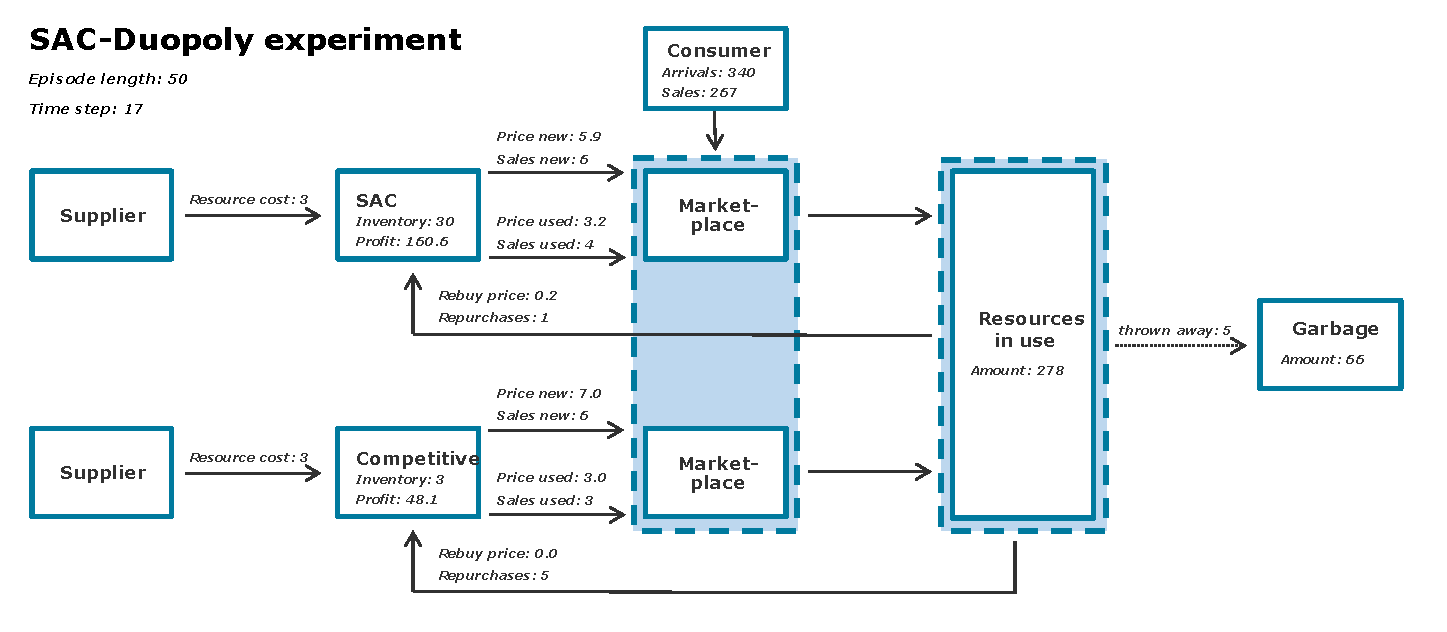
\includegraphics[width = \textwidth]{images/experiments/SACDuopoly/exampleprinter/ExampleprinterStep17.pdf}\\
	\caption{Actions and market states during step 17 of the Exampleprinter session.}\label{fig:SACDuopolyExampleprinter17}
\end{figure}

\subsection{Policyanalyser}\label{subsec:ResultsPolicyanalyser}

After an RL agent has been succesfully trained, or after implementing a new rule-based pricing method, users may want to analyse specific characteristics of the agent's policy using the Policyanalyser. We will show both use cases of the Policyanalyser, by first analysing the policy of our trained SAC-Agent and then analysing the policy of the rule-based \emph{RuleBasedCERebuyAgentStorageMinimizer}. As was explained in \bfref{subsec:Policyanalyser}, we need to define both a marketplace and a template market state before running the Policyanalyser. For our experiments, we used a Circular Economy with rebuy prices, and the following default market state:

\begin{itemize}
	\setlength\itemsep{0em}
	\item Number of products in circulation: 75
	\item Competitor's price for new products: 5
	\item Competitor's price for refurbished products: 3
	\item Competitor's rebuy price: 2
	\item Number of items in own storage: 10
	\item Number of items in competitor's storage: 12
\end{itemize}
In each run, the Policyanalyser will then replace two of those values, as specified by the user, with the features that should be analysed. For our first use case, we will analyse the policy of our trained SAC-Agent. The features that should be replaced are the SAC-Agent's own storage, which will range from 0 to 100, and the competitor's price for refurbished items, ranging from 0 to 10. Note that it does not matter which policy the competitor follows, as the tool does not simulate the market, but only pass market states to the monitored agent. \Cref{fig:PolicyanalyserSAC} shows the respective new and refurbished prices the SAC-Agent would set upon receiving these specific market states.

\begin{figure}[b]
	\centering
	\begin{subfigure}{0.47\textwidth}
		\centering
		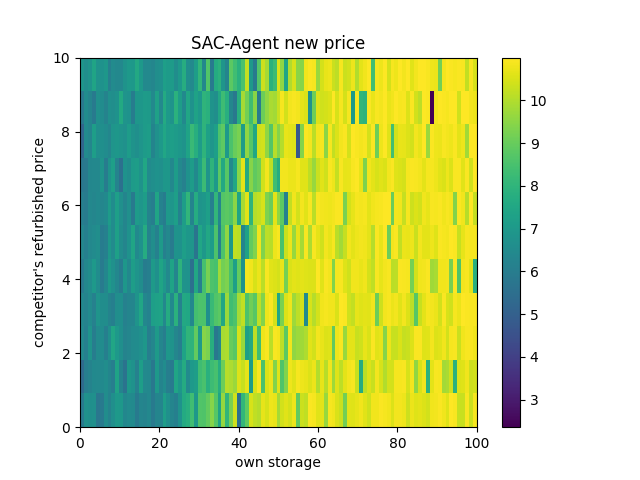
\includegraphics[width = \textwidth]{images/experiments/SACDuopoly/policyanalyzer/SACPolicyanalyzerNewPrice.png}\\
		\subcaption{New prices}\label{fig:PolicyanalyserSAC1}
	\end{subfigure}
	\begin{subfigure}{0.47\textwidth}
		\centering
		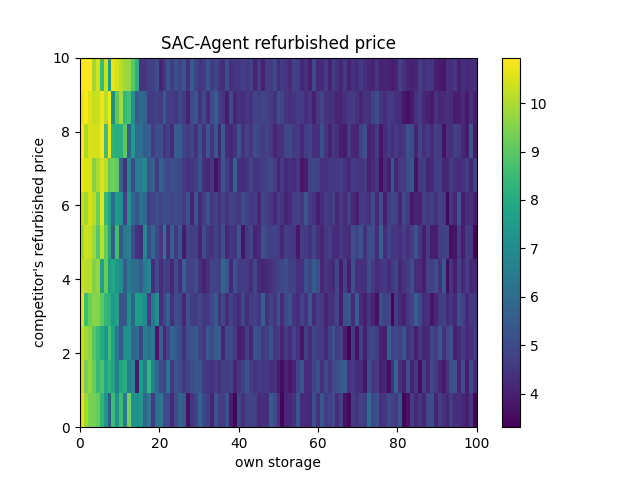
\includegraphics[width = \textwidth]{images/experiments/SACDuopoly/policyanalyzer/SACPolicyanalyzerRefurbishedPrice.png}\\
		\subcaption{Refurbished prices}\label{fig:PolicyanalyserSAC2}
	\end{subfigure}
	\caption{Prices set by the trained SAC-Agent, depending on the competitor's refurbished price and the agent's own storage.}\label{fig:PolicyanalyserSAC}
\end{figure}

From \Cref{fig:PolicyanalyserSAC1} we can infer that the SAC-Agent is not very likely to ever set new prices lower than 6, which coincides with the observed prices set during training, see \Cref{fig:SACDuopolyMixedGraphs4}. \Cref{fig:PolicyanalyserSAC1} also shows that the SAC-Agent will increase prices for new items if it has a higher number of items in its storage, but not necessarily if the competitor's price for refurbished items rises. By increasing the price for new items, the agent tries to de-incentive customers to buy those items from it. At the same time, when looking at \Cref{fig:PolicyanalyserSAC2}, the SAC-Agent will also decrease the price for refurbished items if it has more in storage, again to incentivize customers to buy those products. From both of these diagrams we can see that the SAC-Agent prioritizes making pricing decisions based on the amount of items in its storage, and less based on competitor prices.

Next, we will analyse the policy of the \emph{RuleBasedCERebuyAgentStorageMinimizer} using the Policyanalyser. \Cref{fig:PolicyanalyserRuleBased} shows the results of this monitoring session. \Cref{fig:PolicyanalyserRuleBased1} shows the prices set by the vendor for new products, which follows the agent's policy implementation (see \Cref{fig:PolicyRuleBasedStorageMinimizer}) of always undercutting competitor prices by 1, but always sell above production price (which in this case is 3, see the market configuration file in \Cref{fig:SACDuopolyConfigMarket}).

\Cref{fig:PolicyanalyserRuleBased2} shows the price the rule-based agent will set for buying back items from customers. According to its policy, the rebuy price depends on both the agent's own storage and either its own price for new items (if inventory is low) or competitor's rebuy prices, both of which can be seen nicely in the diagram. As soon as inventory exceeds the limit set in the policy, the agent sets a rebuy price that is 1 lower than the lowest competitor's rebuy price - which in this case is 2, as defined by the template market state. If inventory is low enough, rebuy prices are instead dependent on the vendor's own new prices, as seen in \Cref{fig:PolicyanalyserRuleBased1}, always being one lower, also following the competitor's new price.

\begin{figure}[!t]
	\centering
	\begin{subfigure}{0.47\textwidth}
		\centering
		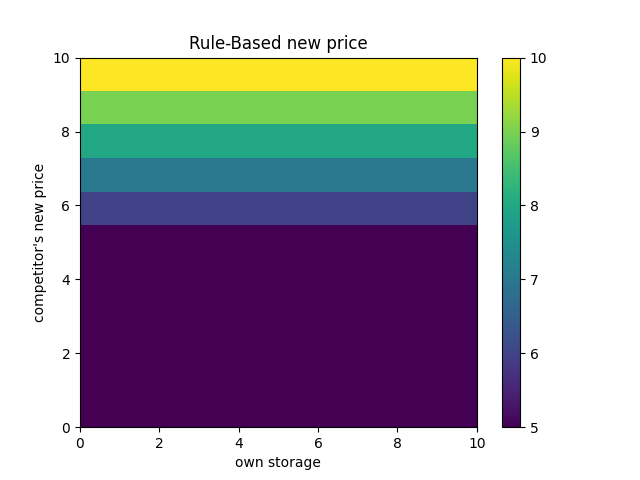
\includegraphics[width = \textwidth]{images/experiments/rulebased/policyanalyzer/RuleBasedPolicyanalyzerNewPrice.png}\\
		\subcaption{New prices}\label{fig:PolicyanalyserRuleBased1}
	\end{subfigure}
	\begin{subfigure}{0.47\textwidth}
		\centering
		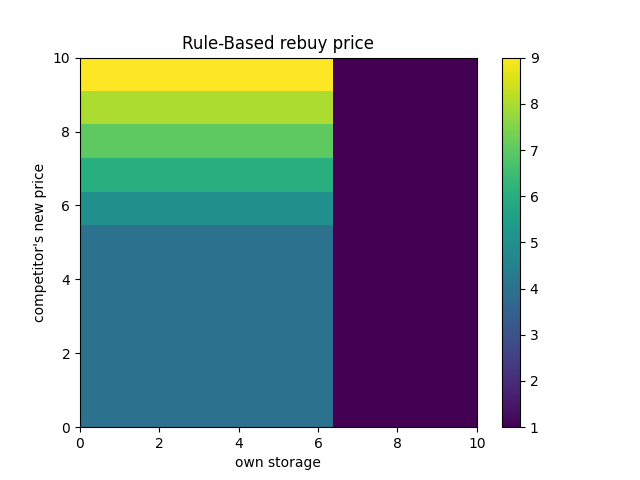
\includegraphics[width = \textwidth]{images/experiments/rulebased/policyanalyzer/RuleBasedPolicyanalyzerRebuyPrice.png}\\
		\subcaption{Rebuy prices}\label{fig:PolicyanalyserRuleBased2}
	\end{subfigure}
	\caption{Prices set by the rule-based agent, depending on the competitor's new price and the agent's own storage.}\label{fig:PolicyanalyserRuleBased}
\end{figure}

\subsection{Other use cases for Agent-monitoring}

Even though most of the diagrams that are created through the Agent-monitoring tool are created if it is run immediately after a training session, it is disconnected from the Live-monitoring tool. There are two major reasons for this, explained in the following two sections.

\subsubsection{Testing rule-based pricing methods}

\begin{figure}[ht]
	\centering
	\begin{subfigure}{0.49\textwidth}
		\centering
		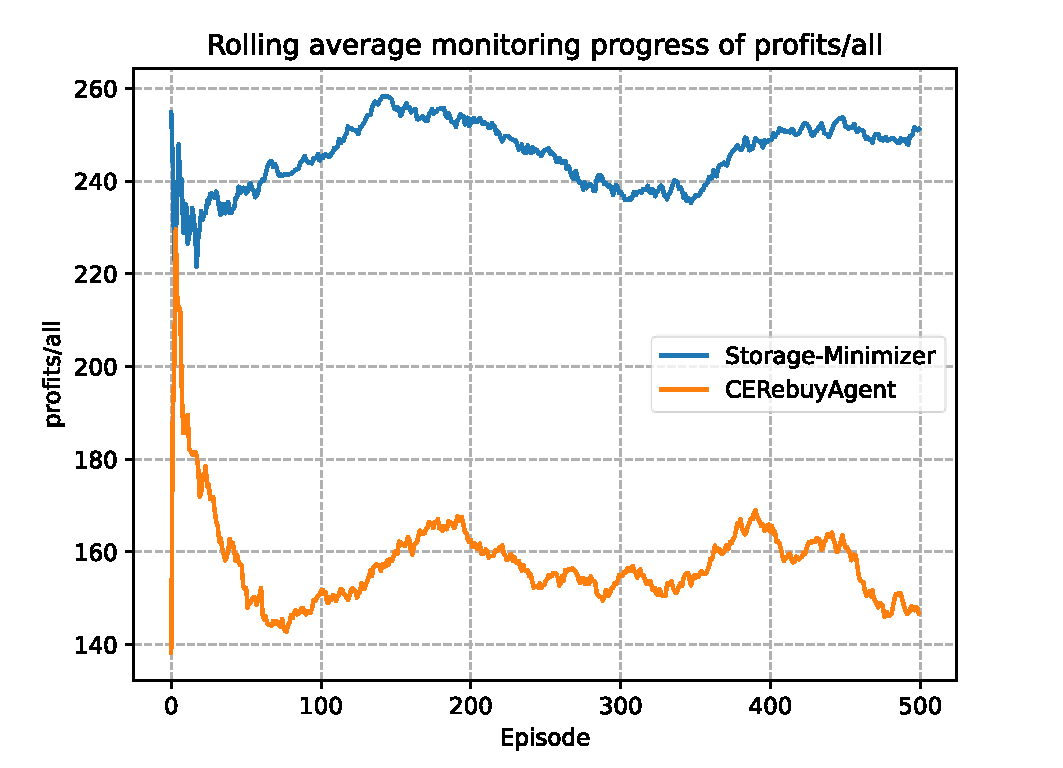
\includegraphics[width = \textwidth]{images/experiments/rulebased/RuleBasedMonitoringProfits.pdf}\\
		\subcaption{Total profits per episode}\label{fig:RulebasedAgentMonitoring1}
	\end{subfigure}
	\begin{subfigure}{0.49\textwidth}
		\centering
		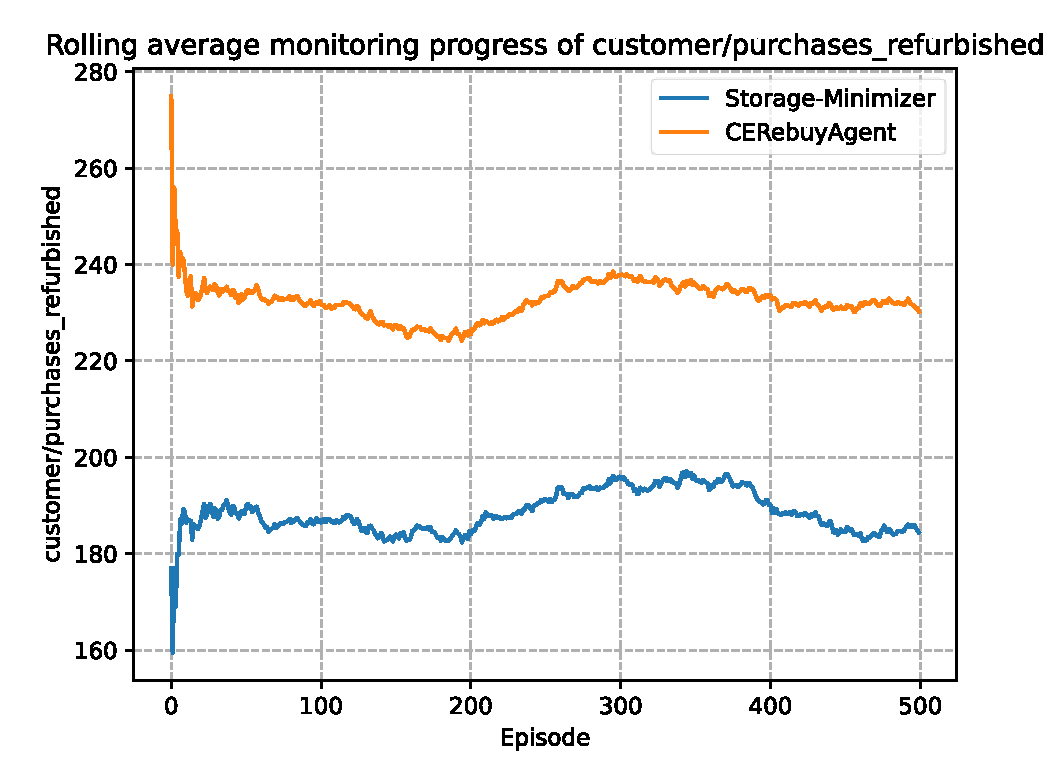
\includegraphics[width = \textwidth]{images/experiments/rulebased/RuleBasedMonitoringPurchasesRefurbished.pdf}\\
		\subcaption{Refurbished products sold per episode}\label{fig:RulebasedAgentMonitoring2}
	\end{subfigure}
	\begin{subfigure}{0.49\textwidth}
		\centering
		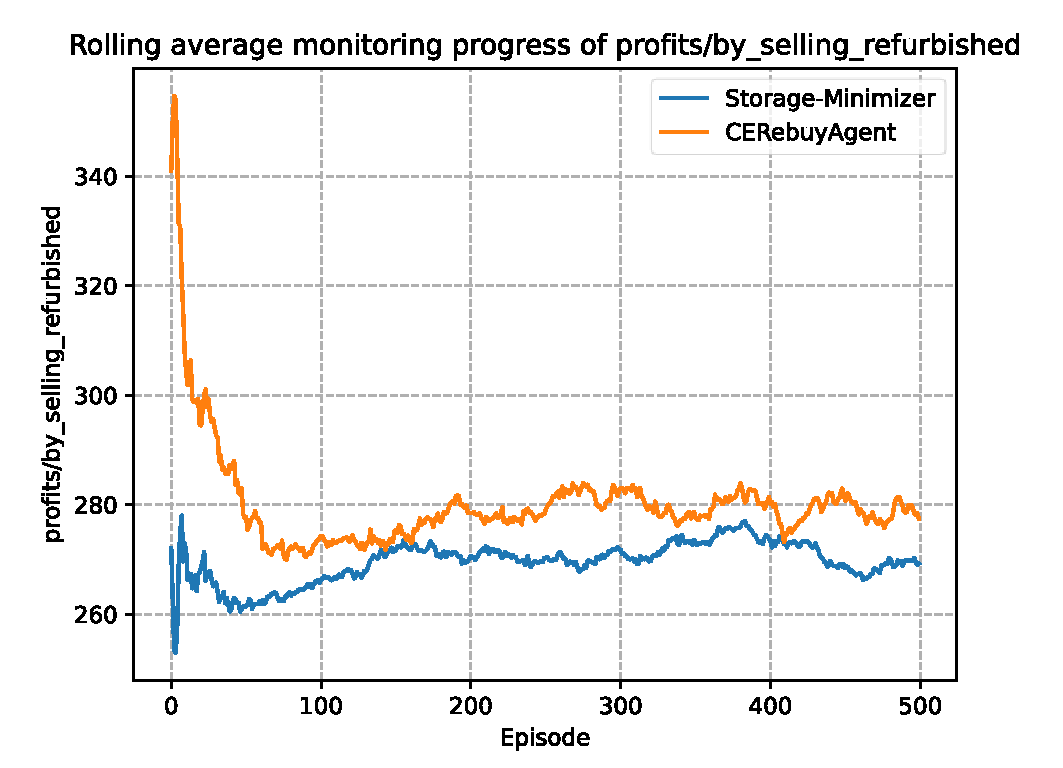
\includegraphics[width = \textwidth]{images/experiments/rulebased/RuleBasedMonitoringProfitsRefurbished.pdf}\\
		\subcaption{Profits by refurbished sales per episode}\label{fig:RulebasedAgentMonitoring3}
	\end{subfigure}
	\caption{Diagrams created during an Agent-monitoring session comparing two rule-based pricing methods.}\label{fig:RulebasedAgentMonitoring}
\end{figure}

First, aside from training RL agents, even though this is the main focus, our market simulation framework can just as well be used to implement and test classically rule-based pricing methods, as we have done ourselves for our rule-based vendors. In order to make this workflow possible, users need to be able to use the Agent-monitoring tool, as it is the only way of running large-scale simulations of different marketplaces aside from training an agent, which is not an option for this use case. \Cref{fig:RulebasedAgentMonitoring} shows the results of an Agent-monitoring session with a \emph{RuleBasedCERebuyAgent} playing against a \emph{RuleBasedCERebuyAgentStorageMinimizer}, a \emph{Data-driven model} that tries to keep the amount of products in its storage as low as possible. Its policy can be found in \Cref{fig:PolicyRuleBasedStorageMinimizer}. As was already mentioned in \bfref{sec:ExplainVendors}, we can see that the \emph{RuleBasedCERebuyAgent} performed significantly worse than the other rule-based agent (\Cref{fig:RulebasedAgentMonitoring1}). This is mainly due to the fact that it is a purely \emph{Inventory-based model}, while the \emph{RuleBasedCERebuyAgentStorageMinimizer} is a \emph{Data-driven} model. Certain characteristics of the \emph{RuleBasedCERebuyAgentStorageMinimizer} can also be seen in \Cref{fig:RulebasedAgentMonitoring2} and \Cref{fig:RulebasedAgentMonitoring3}, as it sells significantly less refurbished products, but is still able to make about the same amount of profits as the simpler \emph{RuleBasedCERebuyAgent}. This can be attributed to its quality of keeping storage costs low by minimizing inventory size.

\subsubsection{Testing trained models against different competitors}

The second reason for having the Agent-monitoring as a stand-alone tool is to be able to monitor trained RL agents not only with the competitors they were trained against, but any combination of other agents, including other trained RL agents. \Cref{fig:SACDuopolyOtherCompetitors} shows this use case on the example of our trained SAC-Agent from the SAC-Duopoly experiment playing not against the \emph{RuleBasedCERebuyAgentCompetitive} it was trained against, but instead playing against a \emph{RuleBasedCERebuyAgentStorageMinimizer}, as introduced in the previous section.

\begin{figure}[t]
	\centering
	\begin{subfigure}{0.49\textwidth}
		\centering
		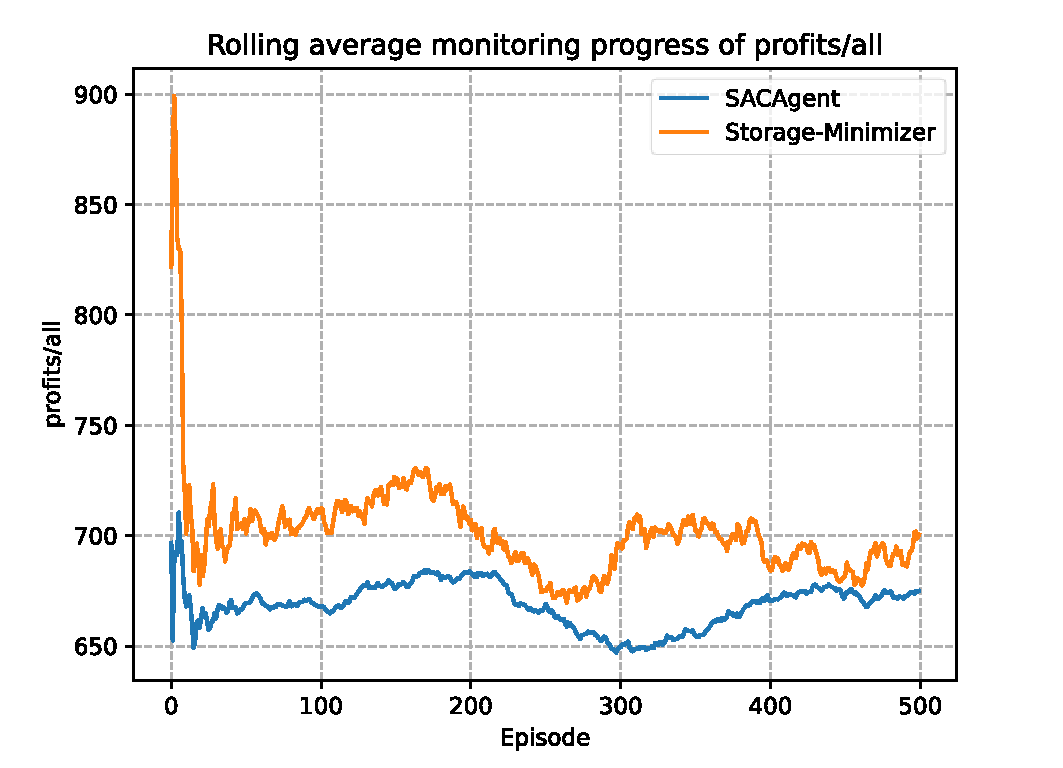
\includegraphics[width = \textwidth]{images/experiments/SACDuopolyOtherComp/SACOtherCompProfitsAll.pdf}\\
		\subcaption{Total profits per episode}\label{fig:SACDuopolyOtherCompetitors1}
	\end{subfigure}
	\begin{subfigure}{0.49\textwidth}
		\centering
		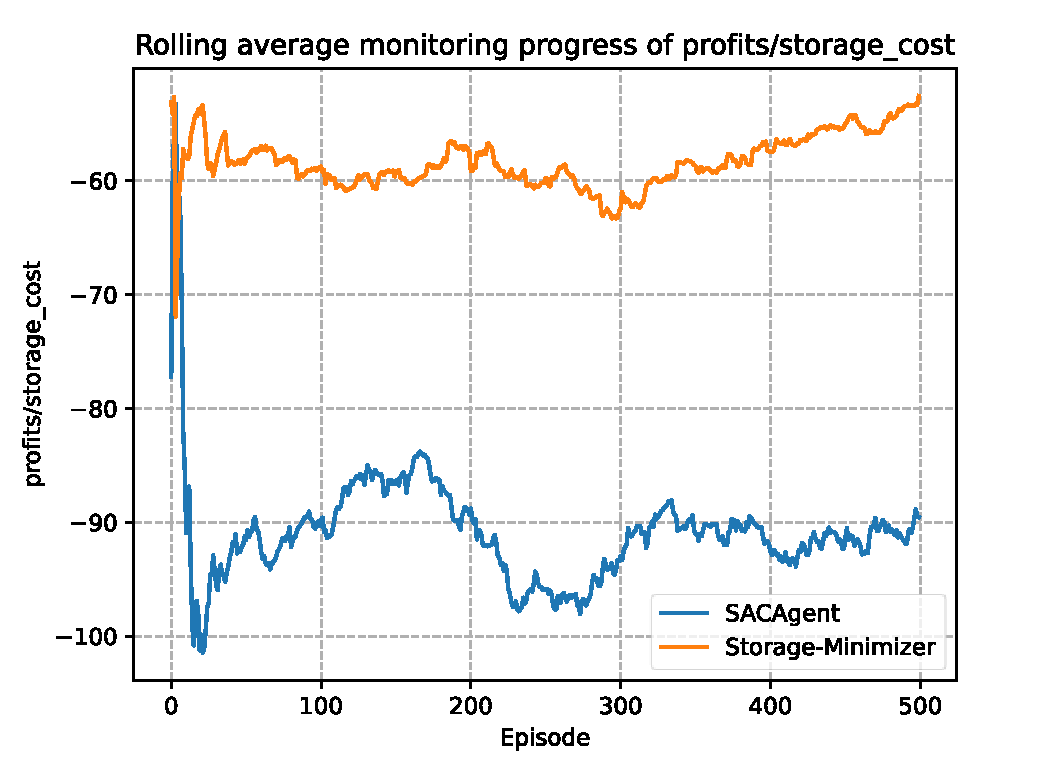
\includegraphics[width = \textwidth]{images/experiments/SACDuopolyOtherComp/SACOtherCompStorageCosts.pdf}\\
		\subcaption{Storage costs per episode}\label{fig:SACDuopolyOtherCompetitors2}
	\end{subfigure}
	\begin{subfigure}{0.49\textwidth}
		\centering
		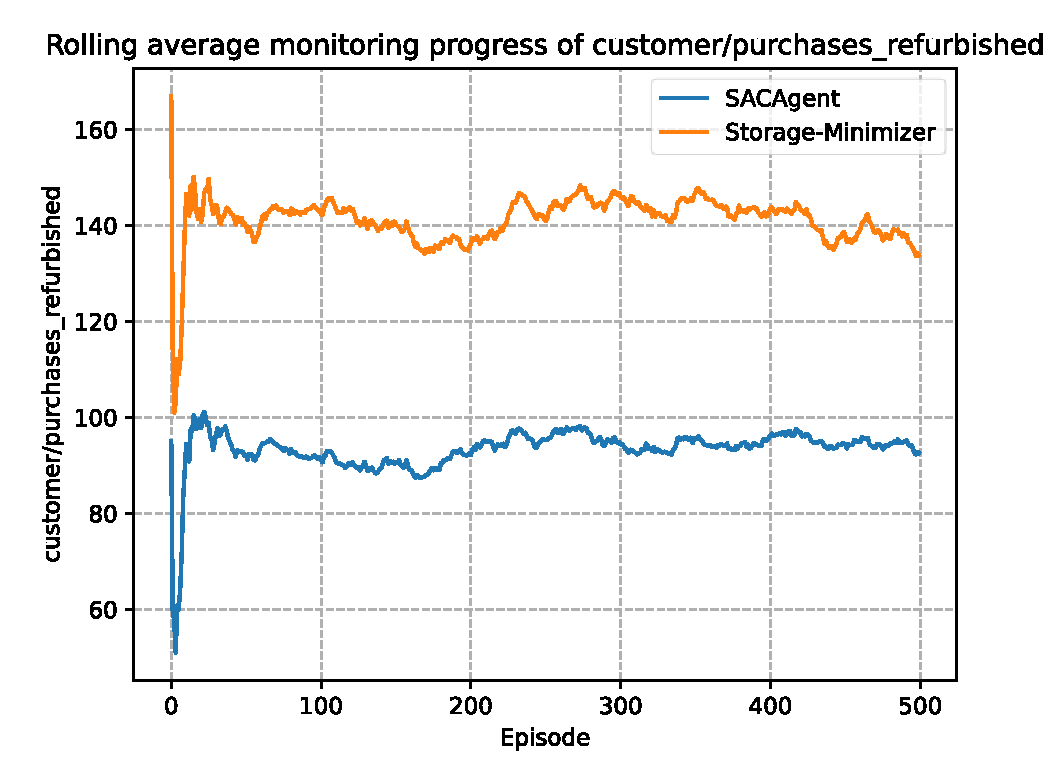
\includegraphics[width = \textwidth]{images/experiments/SACDuopolyOtherComp/SACOtherCompPurchasesRefurbished.pdf}\\
		\subcaption{Sales of refurbished items per episode}\label{fig:SACDuopolyOtherCompetitors3}
	\end{subfigure}
	\caption{Diagrams created during an Agent-monitoring with the SAC-model saved after 1,000 training episodes playing against a \emph{RuleBasedCERebuyAgentStorageMinimizer}.}\label{fig:SACDuopolyOtherCompetitors}
\end{figure}

From \Cref{fig:SACDuopolyOtherCompetitors1} we can infer that the SAC-Agent we trained does not play as well against the \emph{RuleBasedCERebuyAgentStorageMinimizer} as it did against the \emph{RuleBasedCERebuyAgentCompetitive} (\Cref{fig:SACDuopolyProfitsMean1}), as it makes slightly less profits overall and is consistently being outperformed by the rule-based agent. This can be expected, as the trained agent no longer learns the behaviour of its competitor, but now acts according to the previously learned policy. This means that with a change of the competitor, the learned policy may not be as good as it was against the previous opponent.

The impact the different rule-based agent has on the simulation can also be seen in the difference between storage costs of both vendors between the two monitoring runs. While in \Cref{fig:SACDuopolyMixedGraphs1}, both vendors paid storage costs between 50 and 150, this was not the case for the second simulation, where storage costs were much lower for both vendors (\Cref{fig:SACDuopolyOtherCompetitors2}). As the \emph{RuleBasedCERebuyAgentStorageMinimizer} focusses on keeping a low inventory at all times, it also buys back less items. This seems to have agreed with the SAC-Agent's policy, as the trained agent also kept fewer items in inventory in the simulation against this competitor. It was however not able to manage inventory as well as the rule-based agent, as both its storage costs were higher, and sales of refurbished items lower, see \Cref{fig:SACDuopolyOtherCompetitors3}.

% \section*{6.3 Less useful diagrams}\label{sec:UselessDiagrams}

% See todo-note at the top.
% This section is meant to highlight a number of diagrams which are not very useful, such as the `Statistics diagrams'. The reason for this can be twofold: Either the data shown in the diagram is not inertly useful, or the graph provides duplicated or confusing information.